% Preamble:
\documentclass{article}

% Packages:
\usepackage{fancyhdr}
\usepackage{amsmath}
\usepackage{graphicx}
\usepackage{mathbbol}
\usepackage{tikz}
\usetikzlibrary{arrows.meta}
\usetikzlibrary{backgrounds}

% Title Page Information:
\title{CS23 Assignment Seven}
\author{CJ Bridgman-Ford \\ cj.ikaika@gmail.com}
\date{April 23, 2024}

% Make subsections lettered:
\renewcommand{\thesubsection}{\alph{subsection}.}

% fancyhdr Page Styling:
\newcommand{\pagenumber}{\thepage\quad}
\newcommand{\authorname}{CJ Bridgman-Ford}

\pagestyle{fancy}
\renewcommand{\headrulewidth}{0pt}
\fancyhead{}
\fancyfoot[L]{\authorname}
\fancyfoot[C]{}
\fancyfoot[R]{\pagenumber}

% End of Preamble.

% Start of document:
\begin{document}

% Title Page:
\maketitle
\thispagestyle{empty}

\clearpage
% Page 1:
\pagenumbering{arabic}

% Problem 1:

\section{Which of the following graphs contain and Euler path? Which contain and Euler circuit? Show your work (including the graph).}
\subsection{$K_4$}
\hspace{1cm}\textit{$K_4$ does not contain any Euler paths and thus does not contain any Euler circuits. This is because all of the points in the graph have a degree of $3$. An Euler path will only occur in a graph with at most $2$ vertices of odd degree.}
\subsection{$K_5$}
\begin{center}
    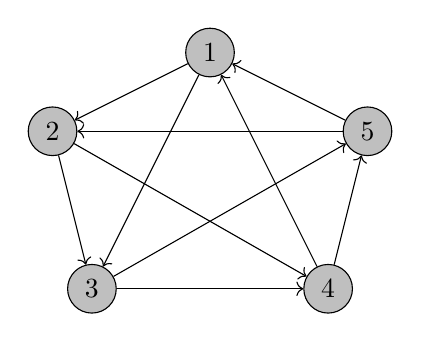
\begin{tikzpicture}[scale=0.5]
        \node[draw, circle, fill=gray!50] (node1) at (-2,4) {1};  
        \node[draw, circle, fill=gray!50] (node2) at (-6,2) {2};
        \node[draw, circle, fill=gray!50] (node3) at (-5,-2) {3};
        \node[draw, circle, fill=gray!50] (node4) at (1,-2) {4};
        \node[draw, circle, fill=gray!50] (node5) at (2,2) {5};
        
        \draw[->] (node1) -- (node3);
        \draw[->] (node3) -- (node5);
        \draw[->] (node5) -- (node2);
        \draw[->] (node2) -- (node4);
        \draw[->] (node4) -- (node1);
        \draw[->] (node1) -- (node2);
        \draw[->] (node2) -- (node3);
        \draw[->] (node3) -- (node4);
        \draw[->] (node4) -- (node5);
        \draw[->] (node5) -- (node1);
    \end{tikzpicture}
\end{center}
\hspace{1cm}\textit{$K_5$ contains an Euler circuit!}
\subsection{$K_{5,7}$}
\hspace{1cm}\textit{$K_{5,7}$ does not contain an Euler path or circuit because all $12$ of the vertices all have odd degrees. This is because $K_{5,7}$ represents a bipartite graph. In the first set, each vertex has $7$ degrees, and in the second set, each vertex has $5$ degrees. This is far beyond the $2$ odd degree vertex limit.}
\clearpage
\subsection{$K_{2,7}$}
\hspace{1cm}\textit{Since $K_{2,7}$ has $2$ vertices with odd degrees, the graph should have an Euler path, but not an Euler circuit. This can be observed inthe below graph where the path can begin on vertex $A$ and end on vertex $B$.}
\begin{center}
    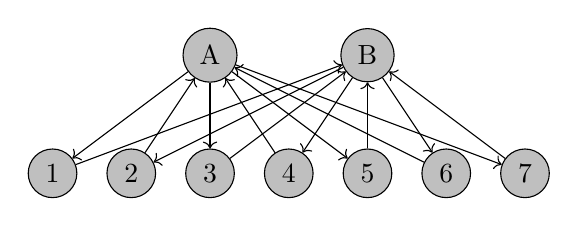
\begin{tikzpicture}
        \node[draw, circle, fill=gray!50] (node1) at (0,0) {1};  
        \node[draw, circle, fill=gray!50] (node2) at (1,0) {2};
        \node[draw, circle, fill=gray!50] (node3) at (2,0) {3};
        \node[draw, circle, fill=gray!50] (node4) at (3,0) {4};
        \node[draw, circle, fill=gray!50] (node5) at (4,0) {5};
        \node[draw, circle, fill=gray!50] (node6) at (5,0) {6};
        \node[draw, circle, fill=gray!50] (node7) at (6,0) {7};
        \node[draw, circle, fill=gray!50] (nodeA) at (2,1.5) {A};
        \node[draw, circle, fill=gray!50] (nodeB) at (4,1.5) {B};
        
        \draw[->] (nodeA) -- (node1);
        \draw[->] (node1) -- (nodeB);
        \draw[->] (nodeB) -- (node2);
        \draw[->] (node2) -- (nodeA);
        \draw[->] (nodeA) -- (node3);
        \draw[->] (node3) -- (nodeB);
        \draw[->] (nodeB) -- (node4);
        \draw[->] (node4) -- (nodeA);
        \draw[->] (nodeA) -- (node5);
        \draw[->] (node5) -- (nodeB);
        \draw[->] (nodeB) -- (node6);
        \draw[->] (node6) -- (nodeA);
        \draw[->] (nodeA) -- (node7);
        \draw[->] (node7) -- (nodeB);
    \end{tikzpicture}
\end{center}
\subsection{$C_7$}
\hspace{1cm}\textit{$C_7$ is cycle graph and therefore contains an Euler circuit. This makes sense because it is a complete graph and every vertex has a degree of $2$.}
\subsection{$P_7$}
\hspace{1cm}\textit{$P_7$ is a graph in which the degrees are $(1,2,2,2,2,2,1)$. Thus, the graph will not have an Euler circuit, but has an euler path. This can be observed in the graph below.}
\begin{center}
    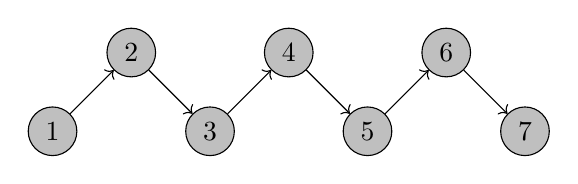
\begin{tikzpicture}
        \node[draw, circle, fill=gray!50] (node1) at (0,0) {1};  
        \node[draw, circle, fill=gray!50] (node2) at (1,1) {2};
        \node[draw, circle, fill=gray!50] (node3) at (2,0) {3};
        \node[draw, circle, fill=gray!50] (node4) at (3,1) {4};
        \node[draw, circle, fill=gray!50] (node5) at (4,0) {5};
        \node[draw, circle, fill=gray!50] (node6) at (5,1) {6};
        \node[draw, circle, fill=gray!50] (node7) at (6,0) {7};
        
        \draw[->] (node1) -- (node2);
        \draw[->] (node2) -- (node3);
        \draw[->] (node3) -- (node4);
        \draw[->] (node4) -- (node5);
        \draw[->] (node5) -- (node6);
        \draw[->] (node6) -- (node7);
    \end{tikzpicture}
\end{center}
\clearpage

% Problem 2:

\section{Consider the following graph:}
\begin{center}
    \includegraphics[scale=0.5]{problem2.png}
\end{center}
\subsection{Find a Hamilton path. Can this path be extended to a Hamilton cycle?}
\hspace{1cm}\textit{I cannot find a hamilton path for this graph. Every path seems to dead end in a two way split. If I could find a path, it could not be extended to a cycle, as the graph appears to be bipartite.}
\begin{center}
    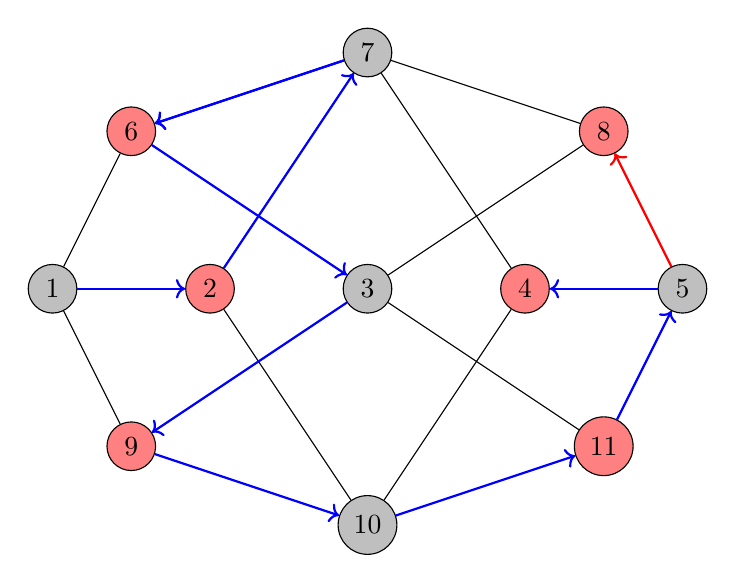
\begin{tikzpicture}
        \node[draw, circle, fill=gray!50] (node1) at (0,0) {1};
        \node[draw, circle, fill=red!50] (node2) at (2,0) {2};
        \node[draw, circle, fill=gray!50] (node3) at (4,0) {3};
        \node[draw, circle, fill=red!50] (node4) at (6,0) {4};
        \node[draw, circle, fill=gray!50] (node5) at (8,0) {5};
        \node[draw, circle, fill=red!50] (node6) at (1,2) {6};
        \node[draw, circle, fill=gray!50] (node7) at (4,3) {7};
        \node[draw, circle, fill=red!50] (node8) at (7,2) {8};
        \node[draw, circle, fill=red!50] (node9) at (1,-2) {9};
        \node[draw, circle, fill=gray!50] (node10) at (4,-3) {10};
        \node[draw, circle, fill=red!50] (node11) at (7,-2) {11};
        
        \draw (node1) -- (node2);
        \draw (node1) -- (node6);
        \draw (node1) -- (node9);
        \draw (node2) -- (node7);
        \draw (node2) -- (node10);
        \draw (node3) -- (node6);
        \draw (node3) -- (node8);
        \draw (node3) -- (node9);
        \draw (node3) -- (node11);
        \draw (node4) -- (node5);
        \draw (node4) -- (node7);
        \draw (node4) -- (node10);
        \draw (node5) -- (node8);
        \draw (node5) -- (node11);
        \draw (node6) -- (node7);
        \draw (node7) -- (node8);
        \draw (node9) -- (node10);
        \draw (node10) -- (node11);
        
        \draw[thick, blue, ->] (node1) -- (node2);
        \draw[thick, blue, ->] (node2) -- (node7);
        \draw[thick, blue, ->] (node7) -- (node6);
        \draw[thick, blue, ->] (node7) -- (node6);
        \draw[thick, blue, ->] (node6) -- (node3);
        \draw[thick, blue, ->] (node3) -- (node9);
        \draw[thick, blue, ->] (node9) -- (node10);
        \draw[thick, blue, ->] (node10) -- (node11);
        \draw[thick, blue, ->] (node11) -- (node5);
        \draw[thick, blue, ->] (node5) -- (node4);
        \draw[thick, red, ->] (node5) -- (node8);
    
    

    \end{tikzpicture}
\end{center}
\clearpage
\subsection{Is the graph bipartite? If so, how many vertices are in each "part"?}
\hspace{1cm}\textit{The graph is bipartite, with $5$ vertices in one part and $6$ in the other.}
\begin{center}
    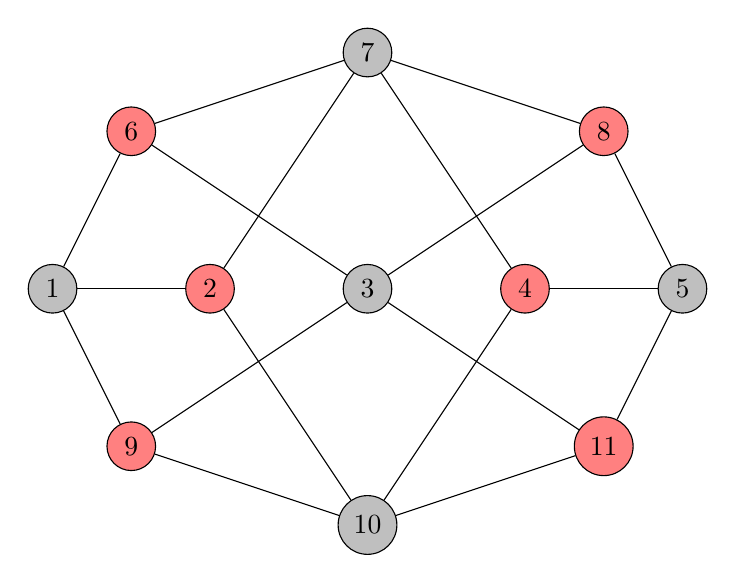
\begin{tikzpicture}
        \node[draw, circle, fill=gray!50] (node1) at (0,0) {1};
        \node[draw, circle, fill=red!50] (node2) at (2,0) {2};
        \node[draw, circle, fill=gray!50] (node3) at (4,0) {3};
        \node[draw, circle, fill=red!50] (node4) at (6,0) {4};
        \node[draw, circle, fill=gray!50] (node5) at (8,0) {5};
        \node[draw, circle, fill=red!50] (node6) at (1,2) {6};
        \node[draw, circle, fill=gray!50] (node7) at (4,3) {7};
        \node[draw, circle, fill=red!50] (node8) at (7,2) {8};
        \node[draw, circle, fill=red!50] (node9) at (1,-2) {9};
        \node[draw, circle, fill=gray!50] (node10) at (4,-3) {10};
        \node[draw, circle, fill=red!50] (node11) at (7,-2) {11};

        \draw (node1) -- (node2);
        \draw (node1) -- (node6);
        \draw (node1) -- (node9);
        \draw (node2) -- (node7);
        \draw (node2) -- (node10);
        \draw (node3) -- (node6);
        \draw (node3) -- (node8);
        \draw (node3) -- (node9);
        \draw (node3) -- (node11);
        \draw (node4) -- (node5);
        \draw (node4) -- (node7);
        \draw (node4) -- (node10);
        \draw (node5) -- (node8);
        \draw (node5) -- (node11);
        \draw (node6) -- (node7);
        \draw (node7) -- (node8);
        \draw (node9) -- (node10);
        \draw (node10) -- (node11);
    \end{tikzpicture}
\end{center}
\subsection{Use your answer in part (b) to prove that the graph has no Hamilton cycle.}
\hspace{1cm}\textit{Since the graph is bipartite, there can only be a Hamilton cycle if the number of vertices in both parts are equal. That is not the case in this graph, therefore, there is no Hamilton cycle.}
\subsection{Suppose you have a bipartite graph $G$ in which one part has at least two more vertices than the other. Prove that $G$ does not have a Hamilton path.}
\hspace{1cm}\textit{A Hamilton path is a bipartite graph will alternate between vertices in the opposing parts. Since the path can only visit each vertex once, there will always be at least $1$ vertex that is impossible to visit.}
\clearpage

% Problem 3:

\section{Find a matching of the bipartite graphs below or explain why no matching exists. Let the graphs be called $A$, $B$, and $C$ from left to right.}
\begin{center}
    \includegraphics[scale=0.33]{problem3.png}
\end{center}
\subsection{Graph $A$:}
\subsection{Graph $B$:}
\subsection{Graph $C$:}
\clearpage

% Problem 4:

\section{What is the smallest number of colors you need to color the vertices of $K_{5,7}$?}
\hspace{1cm}\textit{The smallest number of colors you would need is $2$, since the graph is bipartite.}

% Problem 5:

\section{Draw a graph with chromatic number $5$. \\ Could your graph be planar? Explain.}
\begin{center}
    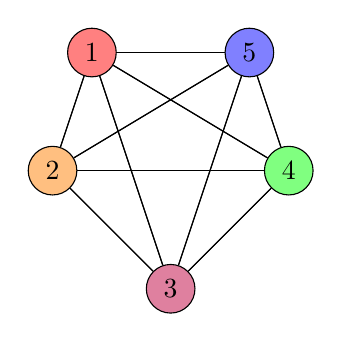
\begin{tikzpicture}
        \node[draw, circle, fill=red!50] (node1) at (-1,1) {1};
        \node[draw, circle, fill=orange!50] (node2) at (-1.5,-0.5) {2};
        \node[draw, circle, fill=purple!50] (node3) at (0,-2) {3};
        \node[draw, circle, fill=green!50] (node4) at (1.5,-0.5) {4};
        \node[draw, circle, fill=blue!50] (node5) at (1,1) {5};

        \draw (node1) -- (node2);
        \draw (node1) -- (node3);
        \draw (node1) -- (node4);
        \draw (node1) -- (node5);
        \draw (node2) -- (node1);
        \draw (node2) -- (node3);
        \draw (node2) -- (node4);
        \draw (node2) -- (node5);
        \draw (node3) -- (node1);
        \draw (node3) -- (node2);
        \draw (node3) -- (node4);
        \draw (node3) -- (node5);
        \draw (node4) -- (node1);
        \draw (node4) -- (node2);
        \draw (node4) -- (node3);
        \draw (node4) -- (node5);
        \draw (node5) -- (node1);
        \draw (node5) -- (node2);
        \draw (node5) -- (node3);
        \draw (node5) -- (node4);
    \end{tikzpicture}
\end{center}
\hspace{1cm}\textit{This graph is not planar as the graph cannot be drawn without edges crossing over.}
\clearpage

% Problem 6:

\section{The local Entomology Club has six work \\ groups, each meeting once a month. How many different meeting times must be used to ensure that no member is scheduled to attend two meetings at the same time if the work groups consist of the following members?}
\begin{center}
    \includegraphics[scale=0.33]{problem6.png}
\end{center}
\begin{center}
    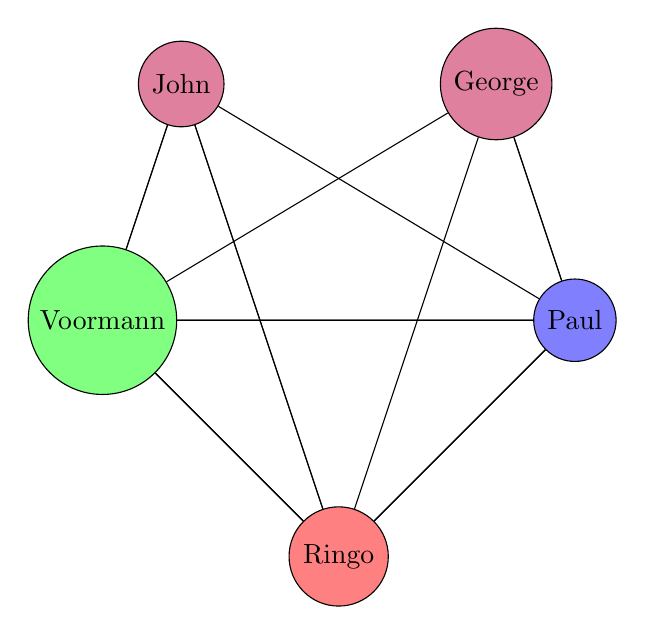
\begin{tikzpicture}[scale=2]
        \node[draw, circle, fill=purple!50] (John) at (-1,1) {John};
        \node[draw, circle, fill=green!50] (Voormann) at (-1.5,-0.5) {Voormann};
        \node[draw, circle, fill=red!50] (Ringo) at (0,-2) {Ringo};
        \node[draw, circle, fill=blue!50] (Paul) at (1.5,-0.5) {Paul};
        \node[draw, circle, fill=purple!50] (George) at (1,1) {George};

        \draw (John) -- (Voormann) -- (Ringo) -- (John);
        \draw (Voormann) -- (George) -- (Paul) -- (Voormann);
        \draw (John) -- (Paul) -- (Ringo) -- (John);
        \draw (George) -- (Paul) -- (Ringo) -- (George);
        \draw (John) -- (Voormann) -- (John);
        \draw (Voormann) -- (Paul) -- (Ringo) -- (Voormann);

    \end{tikzpicture}
\end{center}
\hspace{1cm}\textit{Using a graph where the edges represent who meets with who, and the vertices the individual members, the chromatic number of the graph tells us the number of unique meeting times we need. In this case, the chromatic number is $4$, so we need four different meeting times.}
\clearpage

\end{document}